% ============================================================
% CAPÍTULO 4: METODOLOGIA E EXPERIMENTAÇÃO
% ============================================================
\section{Metodologia e Experimentação}
\label{sec:methodology}

Este capítulo detalha a metodologia utilizada para avaliar o desempenho, a sensibilidade e a robustez à oclusão do estimador proposto. A apresentação segue a ordem lógica dos experimentos: inicialmente, descreve-se a geração cinemática das trajetórias de referência. Em seguida, detalham-se os cenários de teste e a modelagem do filtro. Por fim, definem-se as métricas estatísticas aplicadas na avaliação do Filtro de Kalman Estendido (EKF) sob diferentes parametrizações.

\subsection{Síntese Cinemática das Trajetórias de Referência}
\label{subsec:trajectory_generation}

Para que a precisão do Filtro de Kalman Estendido (EKF) possa ser avaliada, é indispensável compará-lo a um referencial absoluto e livre de ruídos, o \textit{Ground Truth}. Nessa etapa, o simulador atua como um gerador de gabaritos: ele calcula a física exata do alvo para cada instante discreto $k$ e armazena essas informações no vetor de estado $\mathbf{x}_k = [p_{x}, p_{y}, v_{x}, v_{y}, a_{x}, a_{y}]^T$, que engloba as posições, velocidades e acelerações reais nos eixos ortogonais.

Como um alvo em uma aplicação real pode apresentar desde um trajeto altamente previsível até manobras bruscas, o simulador foi projetado para testar os limites do estimador utilizando duas abordagens distintas de movimento:
\begin{itemize}
    \item \textbf{Curvas paramétricas analíticas (Determinísticas):} Simulam cenários onde o alvo obedece a regras geométricas bem definidas e contínuas. Servem para testar o filtro sob dinâmicas estáveis e previsíveis.
    \item \textbf{Modelos numéricos comportamentais (Estocásticos):} Inserem aleatoriedade na navegação do alvo. Servem para testar a capacidade de adaptação do EKF quando o objeto realiza trajetórias erráticas ou mudanças repentinas de direção.
\end{itemize}

O conjunto completo dessas trajetórias, abrangendo todos os perfis cinemáticos abordados nos testes, pode ser visualizado na Figura \ref{fig:trajetorias_simulacao}.

\subsubsection{Geração de Curvas Paramétricas e Analíticas}

Para os testes com movimentos contínuos e regulares, as posições do alvo no simulador são ditadas por funções trigonométricas e hiperbólicas dependentes do tempo. Um cuidado fundamental nessa etapa foi evitar o cálculo numérico das derivadas. Para garantir que o \textit{Ground Truth} seja matematicamente exemplar e livre de erros de discretização, a velocidade e a aceleração do alvo são extraídas a partir da diferenciação analítica exata das equações de posição, conforme detalha o Algoritmo \ref{alg:traj_analitica}.

\begin{algorithm}[h]
\caption{Geração de Trajetórias Paramétricas Analíticas}
\label{alg:traj_analitica}
\begin{algorithmic}[1]
\Require Tempo contínuo $t_k = k \Delta t$, Parâmetros geométricos (Amplitude $A$, Frequência $\omega$)
\For{cada instante $k$}
    \If{Perfil = Circular}
        \State $\mathbf{p}_k \gets [c_x + R\cos(\omega t_k), \; c_y + R\sin(\omega t_k)]^T$
    \ElsIf{Perfil = Mudança de Faixa (Tanh)}
        \State $\mathbf{p}_k \gets [v_x t_k, \; c_y + A\tanh(S \cdot t_k)]^T$
    \ElsIf{Perfil = Lemniscata}
        \State $\mathbf{p}_k \gets [c_x + A\sin(\omega t_k), \; c_y + \frac{A}{2}\sin(2\omega t_k)]^T$
    \EndIf
    
    \State $\mathbf{v}_k \gets \frac{d}{dt}\mathbf{p}_k$
    \State $\mathbf{a}_k \gets \frac{d}{dt}\mathbf{v}_k$
    \State $\mathbf{x}_k \gets [\mathbf{p}_k^T, \mathbf{v}_k^T, \mathbf{a}_k^T]^T$
\EndFor
\Ensure Sequência de estados reais $\mathbf{x}_{1:N}$
\end{algorithmic}
\end{algorithm}

As trajetórias com quinas, como o percurso quadrado, obedecem a esse mesmo rigor determinístico. A única diferença é que a modelagem utiliza segmentos de reta conectados para formar as arestas, aplicando-se uma restrição geométrica de fechamento para garantir que o alvo retorne exatamente à coordenada onde iniciou o percurso.

\subsubsection{Geração de Navegação Aleatória e Oclusões}

\begin{figure*}[t!]
    \centering
    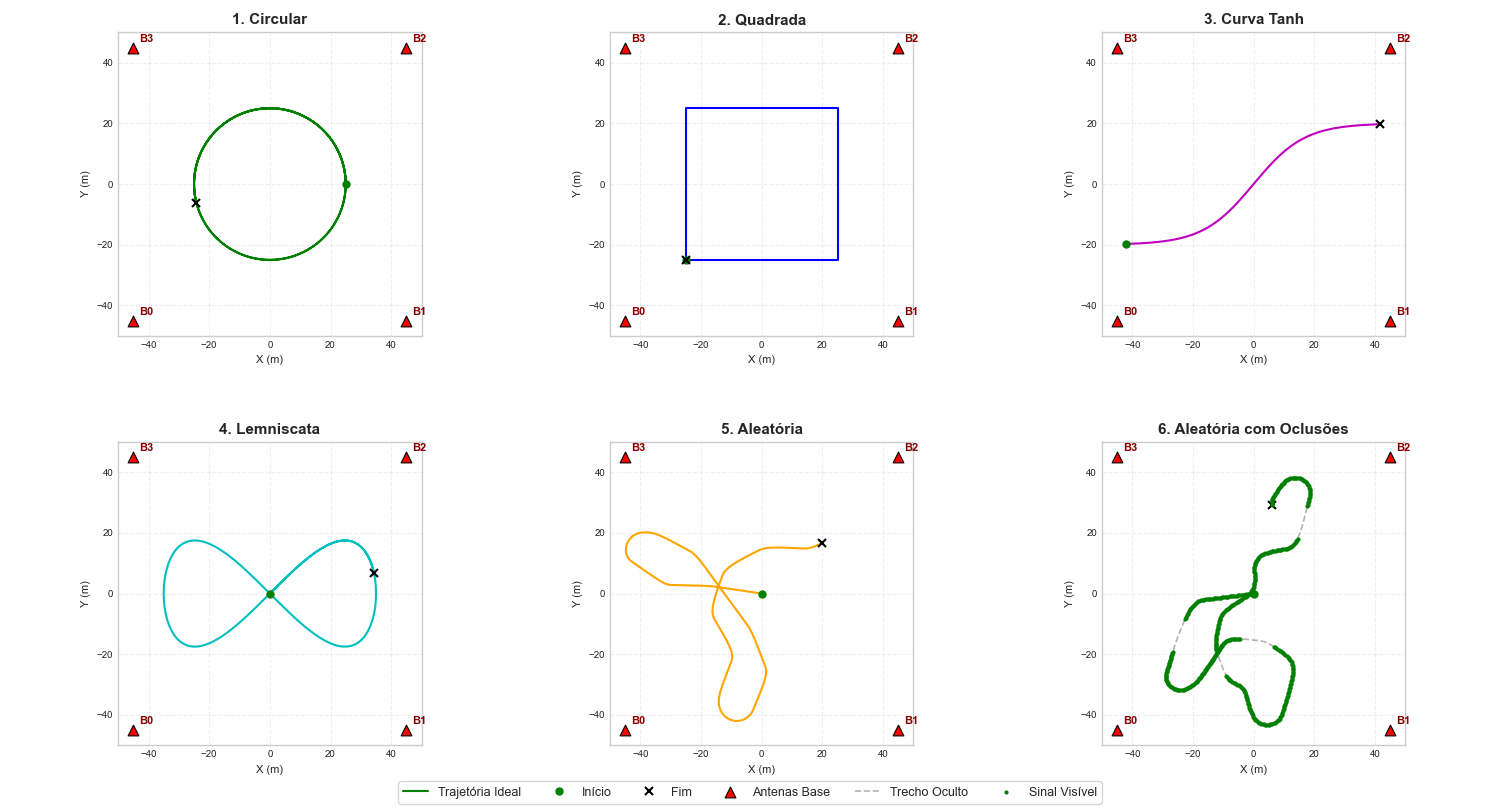
\includegraphics[width=\textwidth]{Figuras/diagrams/trajetorias.png}
    
    \caption{Visualização bidimensional das trajetórias de referência (\textit{Ground Truth}) geradas pelo motor de simulação para a avaliação do estimador sob diferentes perfis cinemáticos.}
    \label{fig:trajetorias_simulacao}
\end{figure*}

Para aproximar a simulação do comportamento estocástico de um alvo real, desenvolveu-se um algoritmo de navegação aleatória. O agente (UGV - Unmanned Ground Vehicle) move-se em linha reta por distâncias mínimas antes de realizar deflexões suaves. Se o robô atinge os limites da arena (raio superior a $35$ metros), um mecanismo de evasão direciona o movimento de volta ao centro, mantendo o robô na área útil.

Como as mudanças de direção são aleatórias, a aceleração de referência é calculada por diferenciação numérica discreta, conforme estruturado no Algoritmo \ref{alg:traj_aleatoria}.

\begin{algorithm}[h]
\caption{Geração de Navegação Dinâmica Aleatória}
\label{alg:traj_aleatoria}
\begin{algorithmic}[1]
\Require Vetor posição central $\mathbf{p}_c$, Limite da arena $R_{\max}$, Ruído cinemático $w$
\For{cada instante $k$}
    \If{Distância percorrida $> D_{\min}$}
        \If{$\|\mathbf{p}_{k-1} - \mathbf{p}_c\| > R_{\max}$}
            \State $\theta_{\text{alvo}} \gets$ Ângulo forçado em direção a $\mathbf{p}_c$
        \Else
            \State $\theta_{\text{alvo}} \gets \theta_{k-1} + \mathcal{U}(-\frac{\pi}{3}, \frac{\pi}{3})$
        \EndIf
        \State $v_{\text{alvo}} \gets v_{\text{base}} + \mathcal{U}(-w, w)$
    \EndIf
    
    \State $\theta_k \gets \text{SuavizarTransição}(\theta_{k-1}, \theta_{\text{alvo}})$
    \State $v_k \gets \text{SuavizarTransição}(v_{k-1}, v_{\text{alvo}})$
    
    \State $\mathbf{v}_k \gets [v_k\cos(\theta_k), \; v_k\sin(\theta_k)]^T$
    \State $\mathbf{p}_k \gets \mathbf{p}_{k-1} + \mathbf{v}_k \Delta t$
    \State $\mathbf{a}_k \gets (\mathbf{v}_k - \mathbf{v}_{k-1}) / \Delta t$
\EndFor

\Statex \textbf{Configuração Especial para Oclusão Cíclica:}
\If{Modo Oclusão}
    \State Emite uma máscara binária atribuindo valor \textit{Falso} (Oculto) no segmento temporal central de 4 blocos.
\EndIf
\end{algorithmic}
\end{algorithm}

\subsection{Cenários de Simulação e Estratégia de Sintonia}
\label{subsec:cenarios_sintonia}

Para avaliar o estimador na prática, a campanha de testes foi dividida em \textbf{6 cenários cinemáticos} (ilustrados na Figura \ref{fig:trajetorias_simulacao}), abrangendo diferentes perfis de aceleração e condições de oclusão. Além do movimento do alvo, o comportamento do EKF depende diretamente das suas matrizes de covariância ($\mathbf{Q}_k$ para o processo e $\mathbf{R}_k$ para a medição). Para testar a robustez e a sensibilidade do algoritmo a esses parâmetros, cada cenário foi avaliado sob \textbf{duas condições de sintonia distintas}:

\begin{enumerate}
    \item \textbf{Situação Sintonizada (Filtro Calibrado):} Representa a condição de funcionamento ideal do rastreador. Os valores das matrizes foram ajustados de forma empírica, baseando-se nas propriedades do ambiente e refinados por tentativa e erro até que o filtro apresentasse o melhor desempenho. A matriz de medição foi definida como $\mathbf{R} = 0,09\mathbf{I}_4$ (quadrado do desvio padrão do ruído das torres, $\sigma = 0,30$ m), enquanto a matriz de processo foi fixada em $\mathbf{Q} = 0,64\mathbf{I}_6$ ($0,8^2$), assumindo estatisticamente as incertezas de modelagem do movimento. O critério de sucesso foi a minimização do erro de posição aliada a elipses de confiança visualmente e estatisticamente coerentes com a trajetória real.
    
    \item \textbf{Situação Não Sintonizada (Filtro Descalibrado):} Representa falhas na configuração do projeto. Nessa etapa, os valores das matrizes foram intencionalmente alterados por superestimação (Sup.) ou subestimação (Sub.). O objetivo de impor essas condições anormais é avaliar a sensibilidade do estimador, demonstrar o impacto do desalinhamento de covariâncias no erro adaptativo e comprovar a importância de uma sintonia rigorosa.
\end{enumerate}

A Tabela \ref{tab:parametros_simulacao} consolida todas as variáveis utilizadas nos testes: a configuração de movimento do alvo, o nível de ruído físico ($\sigma$) simulado nos sensores e os valores numéricos utilizados para sintonizar (ou descalibrar) o EKF em cada um dos seis cenários.

\begin{table*}[t!]
\centering
\caption{Parâmetros de Configuração Cinemática e Sintonia das Matrizes (Mundo Simulado vs. Estimador EKF)}
\label{tab:parametros_simulacao}
\small
\begin{tabular}{lcccccc}
\hline \hline
\textbf{Parâmetro} & \textbf{Cenário 1} & \textbf{Cenário 2} & \textbf{Cenário 3} & \textbf{Cenário 4} & \textbf{Cenário 5} & \textbf{Cenário 6} \\ \hline
\textbf{Perfil} & Circular & Quadrada & Tanh & Lemniscata & Nav. Aleatória & Oclusão Cíclica \\ \addlinespace[1mm]

\textbf{Movimento} & \begin{tabular}{@{}c@{}}$v = 10,0$ m/s \\ $r = 30,0$ m\end{tabular} & \begin{tabular}{@{}c@{}}$v = 10$ m/s \\ $L = 40,0$ m\end{tabular} & \begin{tabular}{@{}c@{}}$A_y = 20,0$ m \\ $v= 10,0$ m/s\end{tabular} & \begin{tabular}{@{}c@{}}$v = 10,0$ m/s \\ $A = 35,0$ m\end{tabular} & \begin{tabular}{@{}c@{}}$v_0 = 8,0$ m/s \\  $\epsilon_v = 0,5$ m/s\end{tabular} & \begin{tabular}{@{}c@{}}$v = 5,0$ m/s \\ 30 fr/oclusão \end{tabular} \\ \addlinespace[2mm]

\multicolumn{7}{c}{\cellcolor{gray!20}\textbf{Variáveis do Ambiente Simulado (Adição de Ruído Físico)}} \\ \addlinespace[1mm]
\textbf{Posição das Torres} & \multicolumn{6}{c}{$B_1[10,10]$; $B_2[190,10]$; $B_3[190,130]$; $B_4[10,130]$} \\ \addlinespace[1mm]
\textbf{Tempo de Simulação} & \multicolumn{6}{c}{40 s} \\ \addlinespace[1mm]
\textbf{Taxa de Quadros (FPS)} & \multicolumn{6}{c}{30} \\ \addlinespace[1mm]
\textbf{Semente Aleatória (\textit{Seed})} & \multicolumn{6}{c}{42} \\ \addlinespace[1mm]
\textbf{Ruído nas Torres ($\sigma$)} & $0,30$ m & $0,30$ m & $0,30$ m & $0,30$ m & $0,30$ m & $0,30$ m \\ \addlinespace[2mm]

\multicolumn{7}{c}{\cellcolor{gray!20}\textbf{Sintonia do EKF: Condição Sintonizada}} \\ \addlinespace[1mm]
\textbf{Matriz Medição $\mathbf{R}_{4\times4}$} & $0,09 \mathbf{I}_{4}$ & $0,09 \mathbf{I}_{4}$ & $0,09 \mathbf{I}_{4}$ & $0,09 \mathbf{I}_{4}$ & $0,09 \mathbf{I}_{4}$ & $0,09 \mathbf{I}_{4}$ \\ \addlinespace[1mm]
\textbf{Matriz Processo $\mathbf{Q}_{6\times6}$} & $0.64\mathbf{I}_{6}$ & $0.64 \mathbf{I}_{6}$ & $0.64 \mathbf{I}_{6}$ & $0.64 \mathbf{I}_{6}$ & $0.64 \mathbf{I}_{6}$ & $0.64 \mathbf{I}_{6}$ \\ \addlinespace[2mm]

\multicolumn{7}{c}{\cellcolor{gray!20}\textbf{Sintonia do EKF: Condição Não Sintonizada}} \\ \addlinespace[1mm]
\textbf{Matriz Medição $\mathbf{R}_{4\times4}$} & \begin{tabular}{@{}c@{}}$0,1 \mathbf{I}_{4}$ \\ (Sup.)\end{tabular} & \begin{tabular}{@{}c@{}}$0,1 \mathbf{I}_{4}$ \\ (Sup.)\end{tabular} & \begin{tabular}{@{}c@{}}$0,01 \mathbf{I}_{4}$ \\ (Sub.)\end{tabular} & $0,09 \mathbf{I}_{4}$ & \begin{tabular}{@{}c@{}}$0,01 \mathbf{I}_{4}$ \\ (Sub.)\end{tabular} & \begin{tabular}{@{}c@{}}$0,01 \mathbf{I}_{4}$ \\ (Sub.)\end{tabular} \\ \addlinespace[1mm]
\textbf{Matriz Processo $\mathbf{Q}_{6\times6}$} & \begin{tabular}{@{}c@{}}$0,01 \mathbf{I}_{6}$ \\ (Sub.)\end{tabular} & \begin{tabular}{@{}c@{}}$0,01 \mathbf{I}_{6}$ \\ (Sub.)\end{tabular} & \begin{tabular}{@{}c@{}}$0,5 \mathbf{I}_{6}$ \\ (Sub.)\end{tabular} & \begin{tabular}{@{}c@{}}$0,3 \mathbf{I}_{6}$ \\ (Sub.)\end{tabular} & \begin{tabular}{@{}c@{}}$0,5 \mathbf{I}_{6}$ \\ (Sub.)\end{tabular} & \begin{tabular}{@{}c@{}}$0,05 \mathbf{I}_{6}$ \\ (Sub.)\end{tabular} \\ \hline \hline

\multicolumn{7}{p{16cm}}{\scriptsize \textit{Nota:} $\mathbf{I}_{n}$ representa a matriz identidade de dimensão $n \times n$, denotando configurações diagonais. A matriz $\mathbf{R}$ apresenta um superdimensionamento conservador intencional ($0,9 \mathbf{I}_{4}$), não refletindo estritamente a variância do ruído injetado ($\sigma^2$). No Cenário 4 (Não Sintonizado), $\mathbf{R}$ foi propositalmente mantido inalterado para isolar e avaliar exclusivamente o efeito da subestimação de $\mathbf{Q}$. (Sup.) = Descalibração por Superestimação; (Sub.) = Descalibração por Subestimação.}
\end{tabular}
\end{table*}

\subsection{Configuração do Estimador e Modelagem do Ruído}
\label{subsec:estimator_config}

O objetivo do filtro é estimar o estado completo do alvo (o vetor PVA $\mathbf{x}_k$, detalhado na Seção \ref{sec:problem_formulation}). Para alimentar o algoritmo, o sistema mede a distância do robô até quatro estações rádio-base fixadas nos cantos da arena.

Como nenhum sensor no mundo real é perfeito, o simulador precisa "sujar" as medidas ideais do \textit{Ground Truth}. Para imitar a imprecisão real, o sistema injeta um erro aleatório em cada canal: soma-se à distância exata um ruído gaussiano branco de média zero e desvio padrão $\sigma$ (valores indicados na Tabela \ref{tab:parametros_simulacao}). 

Isso resulta no vetor de observação $\mathbf{z}_k = [z_{1,k}, z_{2,k}, z_{3,k}, z_{4,k}]^T$, que contém as quatro distâncias ruidosas que o EKF efetivamente recebe como entrada, conforme a Equação (\ref{eq:ruido_interface}):
\begin{equation}
    z_{i,k} = \| \mathbf{p}_k - \mathbf{p}_{i} \| + v_{i,k}, \quad v_{i,k} \sim \mathcal{N}(0, \sigma^2) \quad \forall \quad i = 1, \dots, 4
    \label{eq:ruido_interface}
\end{equation}

É importante destacar que o EKF trabalha diretamente com essas distâncias puras na sua forma não-linear ($\mathbf{z}_k$). No entanto, para que possamos desenhar a posição lida pelos sensores na interface gráfica do simulador, o sistema realiza um cálculo paralelo. Ele pega essas quatro distâncias com ruído e aplica um algoritmo numérico de multilateração por Mínimos Quadrados para estimar uma coordenada cartesiana $\mathbf{m}_k = [m_{x,k}, m_{y,k}]^T$. Essa coordenada 2D serve estritamente como apoio visual para a tela e para a validação externa, não interferindo nas contas do Filtro de Kalman.

\subsection{Ambiente Computacional e Infraestrutura de Simulação}
\label{subsec:software_environment}

\begin{figure}[htbp]
    \centering   
    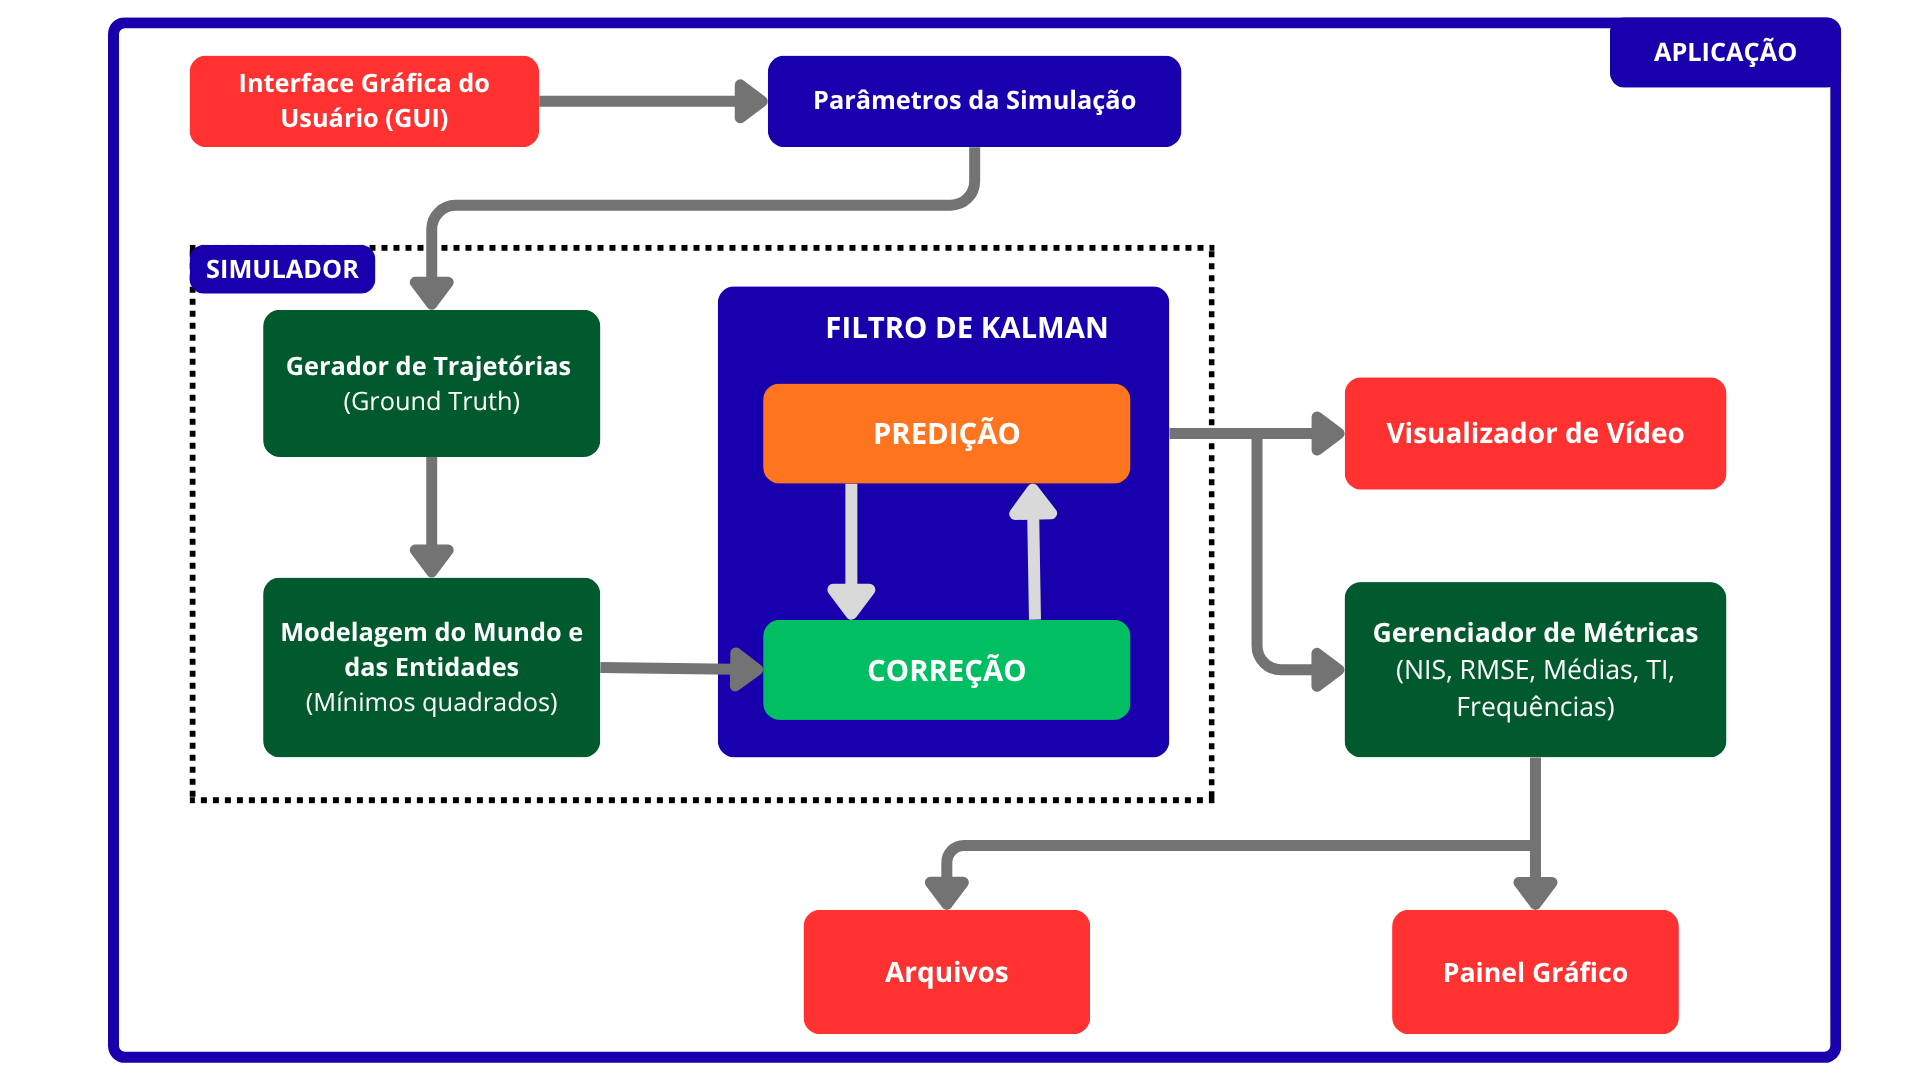
\includegraphics[width=\columnwidth]{Figuras/diagrams/ARQUITETURA.png}
    \caption{Diagrama da arquitetura de software da aplicação de simulação, destacando o fluxo de dados entre o gerador de trajetórias, o estimador de estados e a camada de aplicação.}
    \label{fig:arquitetura_software}
\end{figure}

Para automatizar a execução dos cenários e garantir a reprodutibilidade dos dados, o simulador foi desenvolvido em \textit{Python} (versão 3.10) utilizando uma arquitetura modular, conforme ilustrado na Figura \ref{fig:arquitetura_software}. O processamento matricial e a computação vetorizada do EKF foram implementados com a biblioteca \textit{NumPy}.

Conforme detalhado no diagrama, a arquitetura divide-se logicamente entre o núcleo de simulação e a camada de aplicação. O fluxo de execução inicia-se na Interface Gráfica do Usuário (GUI), onde são definidos os parâmetros iniciais, incluindo a sintonia empírica das matrizes de covariância de processo ($\mathbf{Q}_k$) e de ruído de medição ($\mathbf{R}_k$). Esses parâmetros alimentam o bloco \textit{Simulador}, onde o \textit{Gerador de Trajetórias} estabelece a cinemática real do alvo (\textit{ground truth}). 

Para avaliar adequadamente a capacidade de estimação do filtro, a trajetória exata é ramificada para dois destinos: o \textit{Gerenciador de Métricas} (servindo como base de comparação para o cálculo de erros) e a \textit{Modelagem do Mundo e das Entidades}. Este último atua como o simulador do sistema de localização, convertendo as posições reais em distâncias ruidosas relativas a quatro torres (multilateração). Essa pseudo-observação ruidosa alimenta, então, a etapa de \textit{Correção} do Filtro de Kalman, que trabalha em malha fechada com a \textit{Predição} estocástica.

A GUI, construída nativamente com a biblioteca \textit{Tkinter}, não se limita à parametrização, atuando também na camada de \textit{Aplicação}. Ela integra o \textit{Visualizador de Vídeo} — que renderiza instantaneamente o vetor de observações e a elipse de incerteza da região de interesse (ROI) — e os painéis do \textit{Gerenciador de Métricas}, que acompanham as estatísticas de NIS e RMSE. Apesar dessa integração visual para inspeção qualitativa, o núcleo numérico do simulador opera de forma independente, garantindo que as campanhas de teste em lote e a geração de arquivos de log ocorram de forma assíncrona e automatizada.

\subsection{Métodos de Avaliação e Consistência}
\label{subsec:metricas_metodologia}

O desempenho do EKF é avaliado pela sua precisão espacial e consistência estatística. A acurácia geométrica é quantificada pela Raiz do Erro Quadrático Médio ($\text{RMSE}$), calculada de forma independente para os eixos $X$ e $Y$ ao comparar as estimativas \textit{a posteriori} $(\hat{x}_{k|k}, \hat{y}_{k|k})$ com o \textit{Ground Truth}. O erro médio com sinal ($\text{ME}$) também é monitorado para identificar eventuais vieses sistemáticos no rastreamento.

Embora a análise espacial meça a exatidão geométrica, ela não garante o equilíbrio estatístico do estimador. Para a validação formal de consistência, utiliza-se o \textit{Normalized Innovation Squared} ($\text{NIS}$). O teste do $\text{NIS}$ avalia se a magnitude dos resíduos de inovação é coerente com a incerteza teórica parametrizada nas matrizes de covariância $\mathbf{Q}_k$ e $\mathbf{R}_k$ \cite{barshalom2001estimation}.

\subsubsection{Validação da Crença do Estimador (\textit{Inlier Rate})}
\label{subsubsec:validacao_inliers}

Como métrica complementar em ambiente de simulação, a convergência da crença (\textit{belief}) do filtro é avaliada graficamente pela taxa de \textit{inliers}. Por depender do \textit{Ground Truth}, essa abordagem restringe-se à calibração e análise do comportamento do modelo frente a dados sintéticos controlados.

Baseando-se no conceito de elipsoide de erro \cite{thrun2005probabilistic}, quantifica-se a proporção de frames em que o estado real ($x_{GT}, y_{GT}$) permanece contido na fronteira de incerteza do filtro. A validação baseia-se na distância de Mahalanobis aplicada sobre a submatriz de covariância de posição \textit{a posteriori} $\mathbf{P}_{\text{pos}} = \mathbf{P}_{k|k}^{(1:2, 1:2)}$. Definindo o vetor de erro real como $\tilde{\mathbf{p}}_k = [x_{GT,k} - \hat{x}_{k|k}, \; y_{GT,k} - \hat{y}_{k|k}]^T$, o estado é classificado como um \textit{inlier} se atender à restrição:

\begin{equation}
    \tilde{\mathbf{p}}_k^T \left( \mathbf{P}_{\text{pos}} \right)^{-1} \tilde{\mathbf{p}}_k \le M
    \label{eq:condicao_inlier_quadratica}
\end{equation}
em que $M$ é o valor crítico da distribuição Qui-Quadrado ($\chi^2$) bicaudal com 2 graus de liberdade para o nível de significância adotado.

Para a renderização em tempo real na interface gráfica, a elipse é aproximada por uma janela delimitadora (\textit{bounding box}) baseada no critério $3\sigma$. Os desvios-padrão marginais teóricos são dados por:

\begin{equation}
    \sigma_{x, \text{filt}} = \sqrt{\max(10^{-6}, P_{k|k}^{(1,1)})}
    \label{eq:sigma_x}
\end{equation}
\begin{equation}
    \sigma_{y, \text{filt}} = \sqrt{\max(10^{-6}, P_{k|k}^{(2,2)})}
    \label{eq:sigma_y}
\end{equation}

Os limites semi-eixais da janela visual ($L_x, L_y$) incorporam uma constante de salvaguarda inferior $\tau_{\min}$ para evitar o colapso da caixa em cenários de incerteza nula ou falhas de inicialização:

\begin{equation}
    L_x = \max(\tau_{\min}, 3\sigma_{x,\text{filt}})
    \label{eq:Lx}
\end{equation}
\begin{equation}
    L_y = \max(\tau_{\min}, 3\sigma_{y,\text{filt}})
    \label{eq:Ly}
\end{equation}

A Figura \ref{fig:validacao_inliers} ilustra a correlação espacial entre a elipse probabilística (Equação \ref{eq:condicao_inlier_quadratica}) e a janela ortogonal de renderização (Equações \ref{eq:Lx} e \ref{eq:Ly}), permitindo aferir qualitativamente se a dispersão das estimativas é coerente com a evolução da matriz $\mathbf{P}$.

\subsubsection{Análise de Estabilidade Estatística via Limites de Confiança do NIS}
\label{subsubsec:limites_nis}

Enquanto a taxa de \textit{inliers} atua como um validador visual externo restrito à simulação, o $\text{NIS}$ avalia a estabilidade matemática de forma independente do \textit{Ground Truth}, refletindo a operação real do algoritmo. O teste de hipóteses é governado por um intervalo de confiança bicaudal de 95\%, cujos graus de liberdade ($DOF$) dependem do número de torres de recepção ativas na multilateração a cada passo de tempo $k$.

Para um cenário padrão com 4 graus de liberdade (4 DOF), os limites críticos da tabela $\chi^2$ são $\chi^2_{0.025, 4} = 0{,}484$ (inferior) e $\chi^2_{0.975, 4} = 11{,}143$ (superior). O histórico do $\text{NIS}$ permite classificar o comportamento dinâmico do EKF em três regimes:

\begin{itemize}
    \item \textbf{Filtro Consistente:} O $\text{NIS}$ oscila predominantemente dentro dos limites calculados. Espera-se que aproximadamente 95\% das amostras temporais residam nessa faixa, validando a representação correta da própria incerteza do filtro.
    \item \textbf{Filtro Otimista (Subestimação do Erro):} O $\text{NIS}$ ultrapassa repetidamente o limite superior. Isso indica que os resíduos reais são significativamente maiores do que a covariância calculada em $\mathbf{P}$, sinalizando que o filtro confia excessivamente no modelo preditivo em detrimento das medições, o que gera risco de divergência.
    \item \textbf{Filtro Pessimista (Superestimação do Erro):} O $\text{NIS}$ permanece abaixo do limite inferior. Nesse estado, a matriz de covariância cresce de forma desproporcional aos resíduos de inovação. O filtro torna-se excessivamente conservador e lento para responder a variações dinâmicas do alvo.
\end{itemize}

\begin{figure}[htbp]
    \centering
    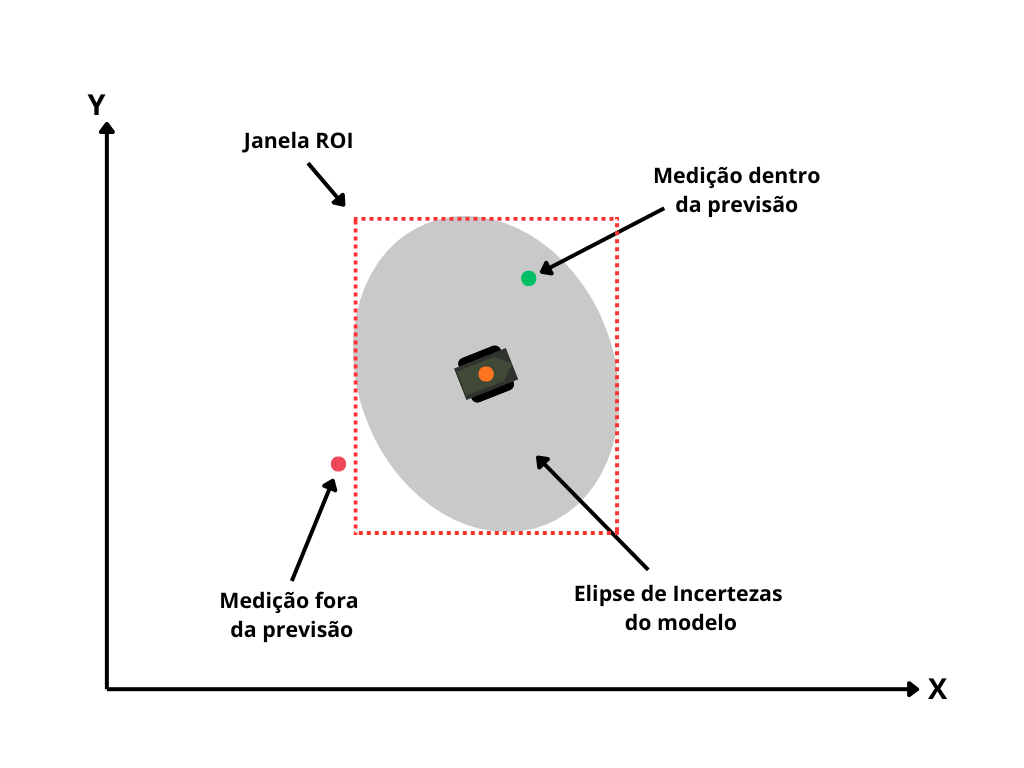
\includegraphics[width=\columnwidth]{Figuras/diagrams/GATTING.png}
    \caption{Representação da métrica de \textit{inliers}. A elipse valida estatisticamente a convergência frente ao Ground Truth, enquanto a janela retangular delimita a incerteza para fins de visualização na GUI.}
    \label{fig:validacao_inliers}
\end{figure}